\subsection{Censored calibration data}\label{sec:res-cens}

Table~\ref{tab:cens} and Fig.~\ref{fig:cens} apply the three censoring mechanisms of the first amendment to the calibration units ($\alpha=0.10$, primary lead time, repetition~0, 50 draws per split). Treating every censored unit as failed immediately after it was last seen alive kept the failure rate at or below its nominal level under every mechanism and censoring fraction on every dataset (H6 supported, 49 of 49 cells), as Theorem~\ref{thm:cens} requires. Whether it was \emph{useful} depended entirely on when units were censored.

When the calibration history came from an earlier alarm at the median critical level, about half of the calibration units (48--51\,\%) were censored, and the censored-as-failure level coincided with the level computed from complete data in every draw at $\alpha=0.10$ (and in 99.3--100\,\% of draws at $\alpha=0.20$): failure rates and notice were identical to the uncensored analysis on all seven datasets. Censoring of this kind, which is what a fleet operated under an alarm produces, cost nothing. Dropping the censored units instead was over-conservative here (failure 2.8--5.5\,\% against 7.0--14.0\,\% uncensored), because the earlier alarm had censored precisely the units with low critical levels.

Under random and administrative censoring, which remove units at arbitrary points of their lives, the guarantee survived but its price was prohibitive: with a quarter of the calibration units censored, the upper bounds of the early-censored units pushed the level to the top of the signal's range, and the alarm fired near the start of life (mean notice at planned replacements 34--751 cycles against 17--46 without censoring). Complete-case calibration stayed close to the uncensored analysis up to half of the units censored (failure 4.5--12.2\,\%), but it carries a guarantee only when censoring is independent of the units (Remark~\ref{rem:cc}), which the administrative mechanism violates by design; with three quarters censored, the 8 remaining calibration units of FD001, FD003 and N-CMAPSS could not certify $\alpha=0.10$ in most draws. The practical reading is that censored fleet data are usable when units are replaced late in life, by an alarm or for reasons unrelated to the units, and that a unit replaced long before an alarm would have acted carries almost no information about how late it could have been replaced.

\begin{table*}[t]\footnotesize\setlength{\tabcolsep}{4pt}
\caption{Censored calibration units ($\alpha=0.10$, primary lead time, repetition~0, mean over 50 censoring draws and five folds): failure before replacement and, in brackets, mean notice at planned replacements (cycles). Policy: history under an earlier alarm at the median critical level (48--51\,\% censored).}\label{tab:cens}
\resizebox{\textwidth}{!}{%
\begin{tabular}{@{}llllllllll@{}}
\toprule
Mechanism & Censored & Method & PHM08 & FD001 & FD002 & FD003 & FD004 & N-CMAPSS & Battery \\
\midrule
None & 0 & complete data & 0.083 (17) & 0.070 (18) & 0.077 (17) & 0.140 (17) & 0.124 (20) & 0.111 (28) & 0.122 (46) \\
Policy & $\approx$\,50\,\% & censored as failure & 0.083 (17) & 0.070 (18) & 0.077 (17) & 0.140 (17) & 0.124 (20) & 0.111 (28) & 0.122 (46) \\
 & & complete case & 0.034 (18) & 0.028 (25) & 0.032 (19) & 0.055 (29) & 0.054 (23) & 0.046 (33) & 0.035 (66) \\
Random & 25\,\% & censored as failure & 0.000 (175) & 0.000 (166) & 0.000 (169) & 0.001 (180) & 0.000 (196) & 0.005 (47) & 0.000 (654) \\
 & & complete case & 0.083 (17) & 0.065 (18) & 0.079 (17) & 0.101 (18) & 0.116 (20) & 0.098 (28) & 0.107 (48) \\
 & 50\,\% & complete case & 0.072 (17) & 0.054 (20) & 0.076 (17) & 0.093 (21) & 0.108 (21) & 0.082 (31) & 0.094 (52) \\
Administrative & 25\,\% & censored as failure & 0.000 (72) & 0.000 (99) & 0.000 (77) & 0.000 (140) & 0.000 (150) & 0.036 (34) & 0.000 (751) \\
 & & complete case & 0.081 (17) & 0.074 (18) & 0.079 (17) & 0.098 (18) & 0.122 (20) & 0.088 (29) & 0.114 (47) \\
 & 50\,\% & complete case & 0.066 (17) & 0.063 (19) & 0.071 (17) & 0.077 (20) & 0.109 (21) & 0.045 (34) & 0.102 (52) \\
\bottomrule
\end{tabular}}
\end{table*}

\begin{figure*}[t]\centering
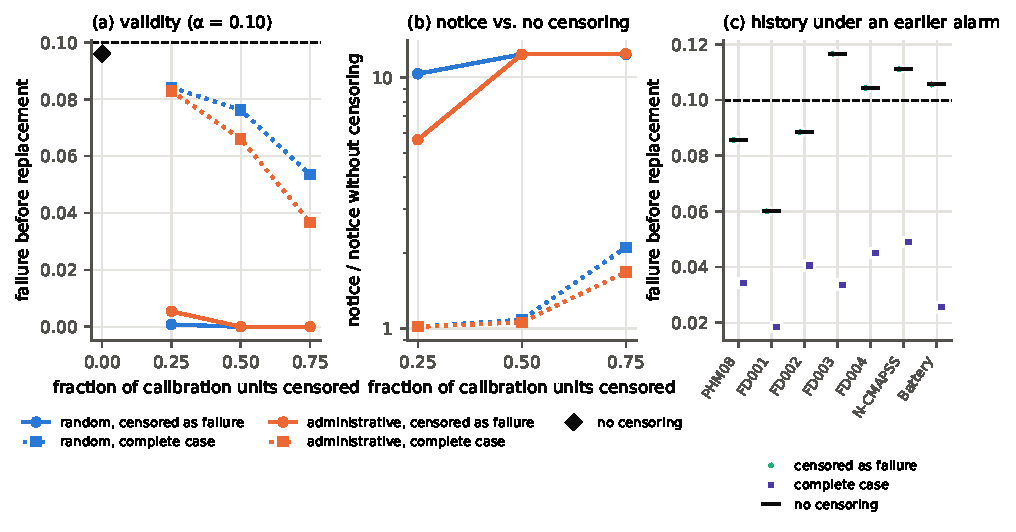
\includegraphics[width=0.95\textwidth]{figures/Fig6_censoring.pdf}
\caption{Censored calibration units ($\alpha=0.10$, primary lead time, repetition~0). (a) Failure before replacement against the fraction of calibration units censored, mean over datasets. (b) Notice relative to the uncensored analysis (log scale). (c) Calibration history produced by an earlier alarm: censored-as-failure reproduces the uncensored result (bars) exactly; complete-case analysis is over-conservative.}\label{fig:cens}
\end{figure*}
